\documentclass[conference]{IEEEtran}
\IEEEoverridecommandlockouts
% The preceding line is only needed to identify funding in the first footnote. If that is unneeded, please comment it out.
\usepackage{cite}
\usepackage{amsmath,amssymb,amsfonts}
\usepackage{graphicx}
\usepackage{textcomp}
\usepackage{xcolor}
\usepackage[hidelinks]{hyperref}


\def\BibTeX{{\rm B\kern-.05em{\sc i\kern-.025em b}\kern-.08em
    T\kern-.1667em\lower.7ex\hbox{E}\kern-.125emX}}
\begin{document}

\title{Conference Paper Title*\\
}

\author{\IEEEauthorblockN{1\textsuperscript{st} Shahriar Kariman }
\IEEEauthorblockA{\textit{dept. name of organization (of Aff.)} \\
\textit{University of New Brunswick}\\
Fredericton, Canada \\
skariman@unb.ca}
\and
\IEEEauthorblockN{2\textsuperscript{nd} Promise Eskor Ononokpono}
\IEEEauthorblockA{\textit{dept. name of organization (of Aff.)} \\
\textit{University of New Brunswick}\\
Fredericton, Canada \\
email address or ORCID}
}

\maketitle

\begin{abstract}
Insert abstract here.
\end{abstract}

\begin{IEEEkeywords}
Put some Key words here.
\end{IEEEkeywords}

\section{Introduction}

With the global transition towards renewable energy and electric vehicles, the demand for lithium-ion batteries is on the rise \cite{b1}. While EV batteries will no longer be able to be used for transportation after reaching 70-80\% of their original battery capacity \cite{b2}. And because EV battery recycling is still very expensive, their reuse is considered to be a more lucrative option as such EV companies have begun to form partnerships with battery manufactures and recycling companies to develop a market around second-life batteries \cite{b3}.

\section{Background}

One of the key factors for a second-life business model is the battery ownership meaning who owns the batteries and decides on the management in the resulting second-life energy system. Currently in most businesses batteries are often obtained through inter-industry partnerships and with government support \cite{b4}.

For a better understanding of the current industry methods with regards to acquiring batteries we looked at 3 successful companies utilizing second-life battery reuse to create a circular economy for batteries.

\begin{table}[htbp]
\caption{Examples of Businesses Utilizing  Second-life}
\begin{center}
\begin{tabular}{|c|c|c|c|}
\hline
\textbf{Company} & \textbf{Business Model} & \textbf{Based In} \\ \hline
Zenobe & EV Manufacturing Company & London \\ \hline
Modual & Battery Repurposing & Switzerland \\ \hline
ECO STORE & Energy Storage Manufacturing Company & Norway \\ \hline
\end{tabular}
\end{center}
\end{table}

All 3 of these companies repurpose used batteries for different second-life applications but they differ in the means of acquiring them, from direct reuse of their own products to partnerships with recycling businesses and government support.

\begin{itemize}
  \item Zenobe reuses end of life batteries from their manufactured electric buses, trucks and commercial vehicles currently in operation \cite{b5}.
  \item Modual purchases batteries and repurposes them for resale in home and business applications \cite{b6}. They also recently secured financing from Switzerland’s Technology Fund to help with their effort \cite{b7}.
  \item ECO STORE acquires the second-life batteries it uses alongside their first-life batteries through their partnership with Morrow and Li-Cycle Holdings which is another battery recycling business \cite{b8, b9}.
\end{itemize}

\subsection{Another Approach}

So far from our research we have established that second-life battery companies have ownership of the batteries they use either as a by-product of their business model or acquire them through transactions and partnerships. We have yet to encounter a case where a business does not own the batteries directly and essentially partners with individual EV owners to reuse their end of life batteries for a cut of the profits, effectively making them shareholders of the business.

But in order for such a business to exist there needs to be an effective and clear way to distribute the profit from the batteries between the business and the battery owners. This is to ensure transparency and trust between all parties involved and satisfaction from the end result.

We propose two potential approaches to profit distribution for such a business:

\begin{enumerate}
    \item The batteries put together in a cluster could have a system alongside them that continuously gathers information on the batteries charge and discharge along with their state of health. That way the contribution of each battery can be definitively calculated and a share of the revenue sent back to the owner.
    \item The batteries could be checked at the beginning and based on the state of health and capacity of the battery assigned a percentage that the owners will receive from the entire cluster. This percentage continues to adjust based on the state of health and capacity of the battery over the course of the simulation.
\end{enumerate}

We aim to model these 2 scenarios to find out which is more profitable and easier to
implement. We hope to shed some light on how a second life battery company should operate
without partnership with other industries or tracking and buying a large number of batteries.

\section{Simulation Design}

For the simulation we assumed that a second-life battery storage system or cluster has 32 batteries. And at the beginning of the simulation we assumed each battery will have an original capacity between 30 to 50 kWh and an initial state of health(SOH) of 60 to 80\% with both capacity and SOH generated randomly.

\begin{equation}
	SOH = \frac{current \ capacity}{original \ capacity}
\end{equation}

In the simulation loop we simulate the use of the batteries for arbitrage over a period of 10 years once for each battery individually and once as all of them managed as part of a storage system of 32 batteries. The arbitrage simulation uses the TOU rates obtained from the Ontario Energy Board \cite{b11}.

For the batteries in the storage system we used a greedy algorithm to distribute the load for each one hour period meaning we sorted the batteries in descending order of state of health and in ascending or descending order of state of charge depending on whether the cluster is charging or discharging.

And based on the outcome of the greedy algorithm we calculated the cycle degradations and calendar degradations using formulas found in an IEEE paper titled “Joint Arbitrage and Operating Reserve Scheduling of Energy Storage Through Optimal Adaptive Allocation of the State of Charge” by Hadi Khani and Hany E. Z. Farag from York University of Toronto \cite{b10}.

Here are the formulas we used to calculate the degredations:

\begin{equation}
\begin{aligned}
	D_{cycle} = K_{cycle} \times \frac{| \Delta E |}{current \ capacity}
\end{aligned}
\end{equation}

\begin{equation}
\begin{aligned}
	D_{calender} = K_{calender} \times \Delta{T}
\end{aligned}
\end{equation}

Where:
\begin{itemize}
    \item \( D_{cycle} \) is the cycle degredation for an hour,
    \item \( D_{calender} \) is the calender degredation for T hours,
    \item \( K_{cycle} \) is the cycle degredation rate per full charge rate equal to $ 4.6 \times 10^{-3}$ , and
    \item \( K_{calender} \) represents the time based degredation rate per hour assuming 2\% annual degredation.
\end{itemize}

After having the degradations the simulation then re-calculates the current capacity based on the same IEEE paper used to calculate the degradations \cite{b10}.

\begin{equation}
\begin{aligned}
	new \ capacity = capacity - total \ degredation
\end{aligned}
\end{equation}

The entire simulation is implemented with object oriented programming principles in mind and it comprises of four main classes for running the simulation as well as some pytests to test the functionality of “battery.py”, “cluster.py” and the decision making algorithm used in “arbitrage\_simulation.py”. Figure 1 shows a class diagram of the simulation.

\begin{figure}[h!]
    \centering
    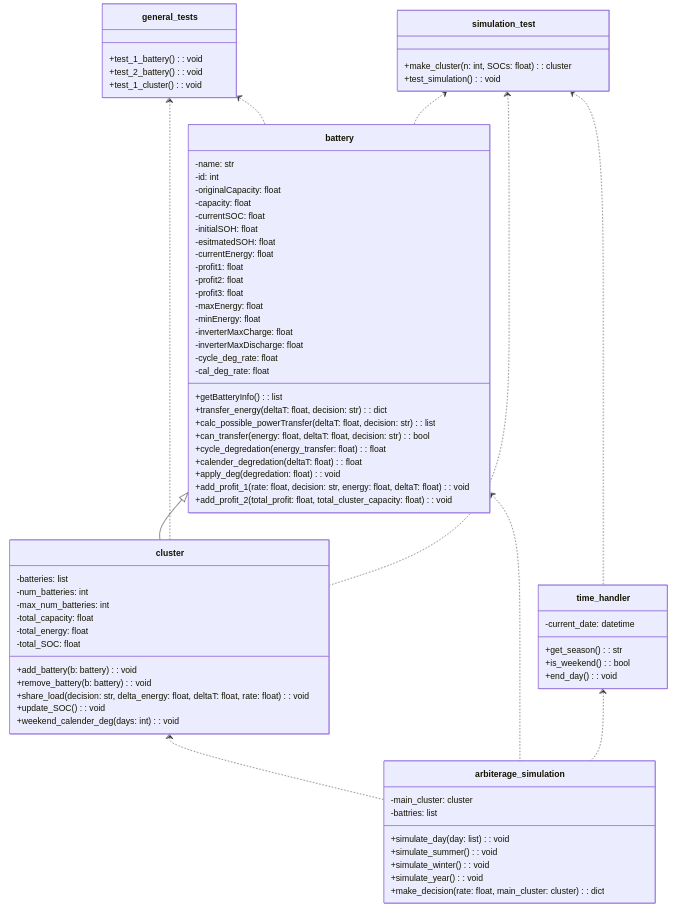
\includegraphics[width=0.5\textwidth]{{img/class_diagram.png}}
    \caption{Class diagram for the simulation.}
    \label{fig:class diagram}
\end{figure}

At the end the simulation results are stored within the battery objects, analyzed using NumPy, and visualized with Plotly.

\section*{Acknowledgment}

% this is were we acknowldge that we both worked equally 

The preferred spelling of the word ``acknowledgment'' in America is without 
an ``e'' after the ``g''. Avoid the stilted expression ``one of us (R. B. 
G.) thanks $\ldots$''. Instead, try ``R. B. G. thanks$\ldots$''. Put sponsor 
acknowledgments in the unnumbered footnote on the first page.

\begin{thebibliography}{00}
\bibitem{b1} Q. Hassan, P. Viktor, T. J. Al-Musawi, B. M. Ali, S. Algburi, H. M. Alzoubi, A. Khudhair Al-Jiboory, A. Z. Sameen, H. M. Salman, and M. Jaszczur, ``The renewable energy role in the global energy transformations,'' \textit{Renewable Energy Focus}, vol. 48, p. 100545, 2024. [Online]. Available: \href{https://www.sciencedirect.com/science/article/abs/pii/S1755008424000097?casa_token=bUNZr0M6nogAAAAA:BW6rOq1yhF3iUOtobThX-tDWVjZDpJL9Hzmk0HS78usaDj24Zq_MftqZLBkgYpIrtdgdilaX}{www.sciencedirect.com/science/article/abs/pii/S1755008424000097}.

\bibitem{b2} A. Keeli and R. K. Sharma, ``Optimal use of second life battery for peak load management and improving the life of the battery,''  \textit{2012 IEEE International Electric Vehicle Conference}, Greenville, SC, USA, 2012, pp. 1--6. doi: \href{https://ieeexplore-ieee-org.proxy.hil.unb.ca/document/6183276}{ieeexplore-ieee-org.proxy.hil.unb.ca/document/6183276}.


\bibitem{b3} Y. Zhao, O. Pohl, A. I. Bhatt, G. E. Collis, P. J. Mahon, T. Rüther, and A. F. Hollenkamp, ``A review on battery market trends, second-life reuse, and recycling,'' \textit{Sustainable Chemistry}, vol. 2, no. 1, pp. 167--205, 2021. doi: \href{https://www.mdpi.com/2673-4079/2/1/11}{www.mdpi.com/2673-4079/2/1/11}.

\bibitem{b4} N. Jiao and S. Evans, ``Business models for sustainability: The case of second-life electric vehicle batteries,'' \textit{Procedia CIRP}, vol. 40, pp. 250--255, 2016. [Online]. Available: \href{https://www.sciencedirect.com/science/article/pii/S2212827116001293}{www.sciencedirect.com/science/article/pii/S2212827116001293}.

\bibitem{b5} Zenobe Energy [Online]. Available: \href{https://www.zenobe.com/our-story/}{www.zenobe.com/our-story/}. [Accessed: Dec. 2024].

\bibitem{b6} Modual, Modual Series Lite [Online]. Available: \href{https://modual.ch/series-lite/}{modual.ch/series-lite/}. [Accessed: Dec. 2024].

\bibitem{b7} Modual, Technology Fund PR [Online]. Available: \href{https://modual.ch/technology-fund-pr/}{modual.ch/technology-fund-pr/}. [Accessed: Dec. 2024].

\bibitem{b8} ECO STOR, Partners [Online]. Available: \href{https://www.eco-stor.com/partners}{www.eco-stor.com/partners}. [Accessed: Dec. 2024].

\bibitem{b9} Li-Cycle and Strategic Partners to Build New Lithium-ion Battery Recycling Facility in Norway, Li-Cycle, Jan. 26, 2022. [Online]. Available: \href{https://investors.li-cycle.com/news/news-details/2022/Li-Cycle--Strategic-Partners-to-Build-New-Lithium-ion-Battery-Recycling-Facility-in-Norway/default.aspx}{https://investors.li-cycle.com/news/news-details/2022/Li-Cycle--Strategic-Partners-to-Build-New-Lithium-ion-Battery-Recycling-Facility-in-Norway/default.aspx}. [Accessed: Dec. 14, 2024].

\bibitem{b10} H. Khani and H. E. Z. Farag, ``Joint Arbitrage and Operating Reserve Scheduling of Energy Storage Through Optimal Adaptive Allocation of the State of Charge,'' \textit{IEEE Trans. Sustainable Energy}, vol. 10, no. 4, pp. 1705--1717, Oct. 2019, doi: \href{https://ieeexplore.ieee.org/document/8463591}{ieeexplore.ieee.org/document/8463591}.

\bibitem{b11}
Ontario Energy Board, ``Electricity rates,'' [Online]. Available: \href{https://www.oeb.ca/consumer-information-and-protection/electricity-rates}{www.oeb.ca/consumer-information-and-protection/electricity-rates}. [Accessed: Dec. 12, 2024].


\end{thebibliography}

\end{document}
